\documentclass[twoside]{book}

% Packages required by doxygen
\usepackage{fixltx2e}
\usepackage{calc}
\usepackage{doxygen}
\usepackage{graphicx}
\usepackage[utf8]{inputenc}
\usepackage{makeidx}
\usepackage{multicol}
\usepackage{multirow}
\PassOptionsToPackage{warn}{textcomp}
\usepackage{textcomp}
\usepackage[nointegrals]{wasysym}
\usepackage[table]{xcolor}

% Font selection
\usepackage[T1]{fontenc}
\usepackage{mathptmx}
\usepackage[scaled=.90]{helvet}
\usepackage{courier}
\usepackage{amssymb}
\usepackage{sectsty}
\renewcommand{\familydefault}{\sfdefault}
\allsectionsfont{%
  \fontseries{bc}\selectfont%
  \color{darkgray}%
}
\renewcommand{\DoxyLabelFont}{%
  \fontseries{bc}\selectfont%
  \color{darkgray}%
}
\newcommand{\+}{\discretionary{\mbox{\scriptsize$\hookleftarrow$}}{}{}}

% Page & text layout
\usepackage{geometry}
\geometry{%
  a4paper,%
  top=2.5cm,%
  bottom=2.5cm,%
  left=2.5cm,%
  right=2.5cm%
}
\tolerance=750
\hfuzz=15pt
\hbadness=750
\setlength{\emergencystretch}{15pt}
\setlength{\parindent}{0cm}
\setlength{\parskip}{0.2cm}
\makeatletter
\renewcommand{\paragraph}{%
  \@startsection{paragraph}{4}{0ex}{-1.0ex}{1.0ex}{%
    \normalfont\normalsize\bfseries\SS@parafont%
  }%
}
\renewcommand{\subparagraph}{%
  \@startsection{subparagraph}{5}{0ex}{-1.0ex}{1.0ex}{%
    \normalfont\normalsize\bfseries\SS@subparafont%
  }%
}
\makeatother

% Headers & footers
\usepackage{fancyhdr}
\pagestyle{fancyplain}
\fancyhead[LE]{\fancyplain{}{\bfseries\thepage}}
\fancyhead[CE]{\fancyplain{}{}}
\fancyhead[RE]{\fancyplain{}{\bfseries\leftmark}}
\fancyhead[LO]{\fancyplain{}{\bfseries\rightmark}}
\fancyhead[CO]{\fancyplain{}{}}
\fancyhead[RO]{\fancyplain{}{\bfseries\thepage}}
\fancyfoot[LE]{\fancyplain{}{}}
\fancyfoot[CE]{\fancyplain{}{}}
\fancyfoot[RE]{\fancyplain{}{\bfseries\scriptsize Generated on Wed Apr 22 2015 15\+:42\+:42 for My Project by Doxygen }}
\fancyfoot[LO]{\fancyplain{}{\bfseries\scriptsize Generated on Wed Apr 22 2015 15\+:42\+:42 for My Project by Doxygen }}
\fancyfoot[CO]{\fancyplain{}{}}
\fancyfoot[RO]{\fancyplain{}{}}
\renewcommand{\footrulewidth}{0.4pt}
\renewcommand{\chaptermark}[1]{%
  \markboth{#1}{}%
}
\renewcommand{\sectionmark}[1]{%
  \markright{\thesection\ #1}%
}

% Indices & bibliography
\usepackage{natbib}
\usepackage[titles]{tocloft}
\setcounter{tocdepth}{3}
\setcounter{secnumdepth}{5}
\makeindex

% Hyperlinks (required, but should be loaded last)
\usepackage{ifpdf}
\ifpdf
  \usepackage[pdftex,pagebackref=true]{hyperref}
\else
  \usepackage[ps2pdf,pagebackref=true]{hyperref}
\fi
\hypersetup{%
  colorlinks=true,%
  linkcolor=blue,%
  citecolor=blue,%
  unicode%
}

% Custom commands
\newcommand{\clearemptydoublepage}{%
  \newpage{\pagestyle{empty}\cleardoublepage}%
}


%===== C O N T E N T S =====

\begin{document}

% Titlepage & ToC
\hypersetup{pageanchor=false,
             bookmarks=true,
             bookmarksnumbered=true,
             pdfencoding=unicode
            }
\pagenumbering{roman}
\begin{titlepage}
\vspace*{7cm}
\begin{center}%
{\Large My Project }\\
\vspace*{1cm}
{\large Generated by Doxygen 1.8.8}\\
\vspace*{0.5cm}
{\small Wed Apr 22 2015 15:42:42}\\
\end{center}
\end{titlepage}
\clearemptydoublepage
\tableofcontents
\clearemptydoublepage
\pagenumbering{arabic}
\hypersetup{pageanchor=true}

%--- Begin generated contents ---
\chapter{Hierarchical Index}
\section{Class Hierarchy}
This inheritance list is sorted roughly, but not completely, alphabetically\+:\begin{DoxyCompactList}
\item \contentsline{section}{fb\+:\+:Face\+Booklet}{\pageref{classfb_1_1_face_booklet}}{}
\item \contentsline{section}{fb\+:\+:I\+Database}{\pageref{structfb_1_1_i_database}}{}
\begin{DoxyCompactList}
\item \contentsline{section}{fb\+:\+:Database}{\pageref{classfb_1_1_database}}{}
\end{DoxyCompactList}
\item \contentsline{section}{fb\+:\+:I\+Face\+Booklet\+Node}{\pageref{structfb_1_1_i_face_booklet_node}}{}
\begin{DoxyCompactList}
\item \contentsline{section}{fb\+:\+:Profile}{\pageref{classfb_1_1_profile}}{}
\end{DoxyCompactList}
\item \contentsline{section}{fb\+:\+:Node\+Data}{\pageref{classfb_1_1_node_data}}{}
\item \contentsline{section}{fb\+:\+:Node\+Post}{\pageref{structfb_1_1_node_post}}{}
\end{DoxyCompactList}

\chapter{Class Index}
\section{Class List}
Here are the classes, structs, unions and interfaces with brief descriptions\+:\begin{DoxyCompactList}
\item\contentsline{section}{\hyperlink{classfb_1_1_database}{fb\+::\+Database} }{\pageref{classfb_1_1_database}}{}
\item\contentsline{section}{\hyperlink{structfb_1_1_date}{fb\+::\+Date} \\*\hyperlink{structfb_1_1_date}{Date} data structure }{\pageref{structfb_1_1_date}}{}
\item\contentsline{section}{\hyperlink{classfb_1_1_face_booklet}{fb\+::\+Face\+Booklet} \\*Main function for \hyperlink{classfb_1_1_face_booklet}{Face\+Booklet} program }{\pageref{classfb_1_1_face_booklet}}{}
\item\contentsline{section}{\hyperlink{structfb_1_1_i_face_booklet_node}{fb\+::\+I\+Face\+Booklet\+Node} \\*Interface class for \hyperlink{classfb_1_1_face_booklet}{Face\+Booklet} nodes }{\pageref{structfb_1_1_i_face_booklet_node}}{}
\item\contentsline{section}{\hyperlink{classfb_1_1_node_data}{fb\+::\+Node\+Data} \\*Class containing a node's basic information and post history.  all \hyperlink{structfb_1_1_i_face_booklet_node}{I\+Face\+Booklet\+Node} types use this class for storing object and post history data. (consider how a Facebook wall is functionally identical for people, groups, and pages.) }{\pageref{classfb_1_1_node_data}}{}
\item\contentsline{section}{\hyperlink{structfb_1_1_node_post}{fb\+::\+Node\+Post} \\*Record type for storing data of a single post }{\pageref{structfb_1_1_node_post}}{}
\item\contentsline{section}{\hyperlink{classfb_1_1_profile}{fb\+::\+Profile} \\*Facebooklet profile class }{\pageref{classfb_1_1_profile}}{}
\item\contentsline{section}{\hyperlink{classfb_1_1_prompter}{fb\+::\+Prompter} \\*Template class for prompting user for data }{\pageref{classfb_1_1_prompter}}{}
\end{DoxyCompactList}

\chapter{File Index}
\section{File List}
Here is a list of all documented files with brief descriptions\+:\begin{DoxyCompactList}
\item\contentsline{section}{/\+Users/\+Shea/cmps/facebooklet/src/{\bfseries Database.\+h} }{\pageref{_database_8h}}{}
\item\contentsline{section}{/\+Users/\+Shea/cmps/facebooklet/src/\hyperlink{_date_8h}{Date.\+h} \\*Date structure type }{\pageref{_date_8h}}{}
\item\contentsline{section}{/\+Users/\+Shea/cmps/facebooklet/src/{\bfseries face.\+h} }{\pageref{face_8h}}{}
\item\contentsline{section}{/\+Users/\+Shea/cmps/facebooklet/src/\hyperlink{_face_booklet_8h}{Face\+Booklet.\+h} \\*Defines main Facebooklet class }{\pageref{_face_booklet_8h}}{}
\item\contentsline{section}{/\+Users/\+Shea/cmps/facebooklet/src/\hyperlink{_f_b_profile_8h}{F\+B\+Profile.\+h} \\*Definition for concrete Profile type }{\pageref{_f_b_profile_8h}}{}
\item\contentsline{section}{/\+Users/\+Shea/cmps/facebooklet/src/\hyperlink{interfaces_8h}{interfaces.\+h} \\*Defines interface type for Facebooklet Nodes }{\pageref{interfaces_8h}}{}
\item\contentsline{section}{/\+Users/\+Shea/cmps/facebooklet/src/\hyperlink{_node_data_8h}{Node\+Data.\+h} \\*Data for building node data }{\pageref{_node_data_8h}}{}
\item\contentsline{section}{/\+Users/\+Shea/cmps/facebooklet/src/\hyperlink{utils_8h}{utils.\+h} \\*Utilitiy functions }{\pageref{utils_8h}}{}
\end{DoxyCompactList}

\chapter{Class Documentation}
\hypertarget{classfb_1_1_database}{\section{fb\+:\+:Database Class Reference}
\label{classfb_1_1_database}\index{fb\+::\+Database@{fb\+::\+Database}}
}
\subsection*{Public Member Functions}
\begin{DoxyCompactItemize}
\item 
\hypertarget{classfb_1_1_database_a6ea6c4bc9187969306785b351891a876}{\hyperlink{classfb_1_1_database_a6ea6c4bc9187969306785b351891a876}{Database} (\hyperlink{classfb_1_1_database}{Database} const \&db)}\label{classfb_1_1_database_a6ea6c4bc9187969306785b351891a876}

\begin{DoxyCompactList}\small\item\em copy constructor \end{DoxyCompactList}\item 
\hypertarget{classfb_1_1_database_a08fa4cc0b0746a3af74bc8b475c816fa}{\hyperlink{classfb_1_1_database}{Database} {\bfseries operator=} (\hyperlink{classfb_1_1_database}{Database} const \&db)}\label{classfb_1_1_database_a08fa4cc0b0746a3af74bc8b475c816fa}

\item 
\hypertarget{classfb_1_1_database_a37037408e2ece4145b6d5487b3fff140}{\hyperlink{structfb_1_1_i_face_booklet_node}{I\+Face\+Booklet\+Node} $\ast$ {\bfseries get\+\_\+node} (id\+\_\+t id)}\label{classfb_1_1_database_a37037408e2ece4145b6d5487b3fff140}

\item 
\hypertarget{classfb_1_1_database_a6c7d28b50a83abc53dea5957231cba36}{\hyperlink{structfb_1_1_i_face_booklet_node}{I\+Face\+Booklet\+Node} $\ast$ {\bfseries new\+\_\+node} (\hyperlink{structfb_1_1_i_face_booklet_node}{I\+Face\+Booklet\+Node} $\ast$node)}\label{classfb_1_1_database_a6c7d28b50a83abc53dea5957231cba36}

\item 
\hypertarget{classfb_1_1_database_a33759a955ab671e0fe014d478250cdc2}{\hyperlink{structfb_1_1_i_face_booklet_node}{I\+Face\+Booklet\+Node} $\ast$ {\bfseries set\+\_\+node} (id\+\_\+t id, \hyperlink{structfb_1_1_i_face_booklet_node}{I\+Face\+Booklet\+Node} $\ast$node)}\label{classfb_1_1_database_a33759a955ab671e0fe014d478250cdc2}

\item 
\hypertarget{classfb_1_1_database_a92c3028d238865d57c94881431465e76}{bool {\bfseries has\+\_\+node} (id\+\_\+t id)}\label{classfb_1_1_database_a92c3028d238865d57c94881431465e76}

\item 
\hypertarget{classfb_1_1_database_ab2ccc687a520e876da67f6620b75308c}{void {\bfseries remove\+\_\+node} (id\+\_\+t id)}\label{classfb_1_1_database_ab2ccc687a520e876da67f6620b75308c}

\item 
\hypertarget{classfb_1_1_database_a94dc36e64c814292188de74e6da46024}{std\+::vector$<$ id\+\_\+t $>$ {\bfseries ids\+\_\+with\+\_\+name} (std\+::string name)}\label{classfb_1_1_database_a94dc36e64c814292188de74e6da46024}

\item 
\hypertarget{classfb_1_1_database_acd72daebc473b882f1a29a288aa13e69}{\hyperlink{classfb_1_1_profile}{Profile} $\ast$ {\bfseries insert\+\_\+profile} (std\+::string const \&name, time\+\_\+t creation\+\_\+time, \hyperlink{structfb_1_1_date}{Date} const \&birthday=\hyperlink{structfb_1_1_date}{Date}(1, Month\+::\+Jan, 1970))}\label{classfb_1_1_database_acd72daebc473b882f1a29a288aa13e69}

\end{DoxyCompactItemize}


The documentation for this class was generated from the following files\+:\begin{DoxyCompactItemize}
\item 
/\+Users/\+Shea/\+Documents/school/cmps/facebooklet/src/\hyperlink{_database_8h}{Database.\+h}\item 
/\+Users/\+Shea/\+Documents/school/cmps/facebooklet/src/Database.\+cc\end{DoxyCompactItemize}

\hypertarget{structfb_1_1_date}{\section{fb\+:\+:Date Struct Reference}
\label{structfb_1_1_date}\index{fb\+::\+Date@{fb\+::\+Date}}
}


\hyperlink{structfb_1_1_date}{Date} data structure.  




{\ttfamily \#include $<$Date.\+h$>$}

\subsection*{Public Member Functions}
\begin{DoxyCompactItemize}
\item 
\hypertarget{structfb_1_1_date_afd4b4fd1e4f19641bd5af1814e28740e}{{\bfseries Date} (time\+\_\+t day=1, Month month=Month\+::\+Jan, time\+\_\+t year=1970)}\label{structfb_1_1_date_afd4b4fd1e4f19641bd5af1814e28740e}

\end{DoxyCompactItemize}
\subsection*{Public Attributes}
\begin{DoxyCompactItemize}
\item 
\hypertarget{structfb_1_1_date_aca51bed7ced0ec90a00380daca6d1774}{time\+\_\+t {\bfseries day}}\label{structfb_1_1_date_aca51bed7ced0ec90a00380daca6d1774}

\item 
\hypertarget{structfb_1_1_date_a67d62b4fd9c0050ffec876eb454719bc}{Month {\bfseries month}}\label{structfb_1_1_date_a67d62b4fd9c0050ffec876eb454719bc}

\item 
\hypertarget{structfb_1_1_date_a8b6c7c2160099c91acb1b573b4a001b8}{time\+\_\+t {\bfseries year}}\label{structfb_1_1_date_a8b6c7c2160099c91acb1b573b4a001b8}

\end{DoxyCompactItemize}


\subsection{Detailed Description}
\hyperlink{structfb_1_1_date}{Date} data structure. 

Simple record type. Should be used as a value type, rather than an abstract object


\begin{DoxyParams}{Parameters}
{\em day} & Must be value greater than one T\+O\+D\+O\+: limit date parameter to valid days in relavent month \\
\hline
{\em month} & month value \\
\hline
{\em year} & year \\
\hline
\end{DoxyParams}


The documentation for this struct was generated from the following files\+:\begin{DoxyCompactItemize}
\item 
/\+Users/\+Shea/\+Documents/school/cmps/facebooklet/src/\hyperlink{_date_8h}{Date.\+h}\item 
/\+Users/\+Shea/\+Documents/school/cmps/facebooklet/src/Date.\+cc\end{DoxyCompactItemize}

\hypertarget{classfb_1_1_face_booklet}{\section{fb\+:\+:Face\+Booklet Class Reference}
\label{classfb_1_1_face_booklet}\index{fb\+::\+Face\+Booklet@{fb\+::\+Face\+Booklet}}
}
\subsection*{Public Member Functions}
\begin{DoxyCompactItemize}
\item 
\hypertarget{classfb_1_1_face_booklet_a9423083c143d839392c89a0e5753bf61}{{\bfseries Face\+Booklet} (\hyperlink{classfb_1_1_face_booklet}{Face\+Booklet} \&)=delete}\label{classfb_1_1_face_booklet_a9423083c143d839392c89a0e5753bf61}

\item 
\hypertarget{classfb_1_1_face_booklet_a59e4c9ecf6767a14f9b79d4f6cfa2c6d}{void {\bfseries run} ()}\label{classfb_1_1_face_booklet_a59e4c9ecf6767a14f9b79d4f6cfa2c6d}

\end{DoxyCompactItemize}


The documentation for this class was generated from the following files\+:\begin{DoxyCompactItemize}
\item 
/\+Users/\+Shea/cmps/facebooklet/src/Face\+Booklet.\+h\item 
/\+Users/\+Shea/cmps/facebooklet/src/Face\+Booklet.\+cc\end{DoxyCompactItemize}

\hypertarget{structfb_1_1_i_face_booklet_node}{\section{fb\+:\+:I\+Face\+Booklet\+Node Struct Reference}
\label{structfb_1_1_i_face_booklet_node}\index{fb\+::\+I\+Face\+Booklet\+Node@{fb\+::\+I\+Face\+Booklet\+Node}}
}


interface class for \hyperlink{classfb_1_1_face_booklet}{Face\+Booklet} nodes  




{\ttfamily \#include $<$I\+Node.\+h$>$}

Inheritance diagram for fb\+:\+:I\+Face\+Booklet\+Node\+:\begin{figure}[H]
\begin{center}
\leavevmode
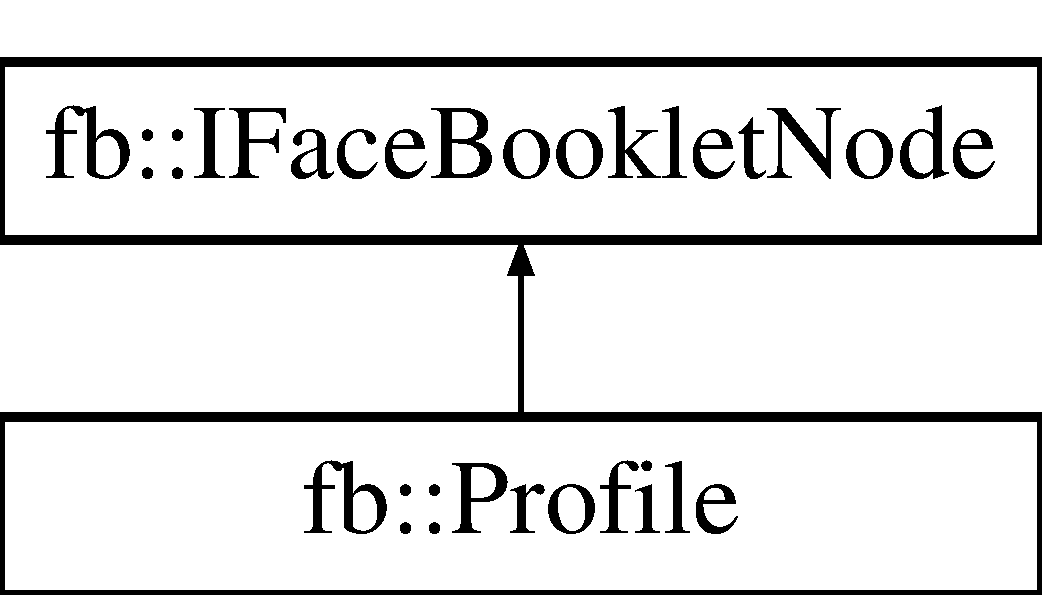
\includegraphics[height=2.000000cm]{structfb_1_1_i_face_booklet_node}
\end{center}
\end{figure}
\subsection*{Public Member Functions}
\begin{DoxyCompactItemize}
\item 
\hypertarget{structfb_1_1_i_face_booklet_node_a9bc90104d8cb2953baee204811aab1cf}{virtual \hyperlink{structfb_1_1_i_face_booklet_node}{I\+Face\+Booklet\+Node} $\ast$ \hyperlink{structfb_1_1_i_face_booklet_node_a9bc90104d8cb2953baee204811aab1cf}{heap\+\_\+copy} ()=0}\label{structfb_1_1_i_face_booklet_node_a9bc90104d8cb2953baee204811aab1cf}

\begin{DoxyCompactList}\small\item\em returns a copy of the node allocated via new() \end{DoxyCompactList}\item 
virtual const id\+\_\+t \hyperlink{structfb_1_1_i_face_booklet_node_a651a6fb7445f8d2c046066c1d381f424}{get\+\_\+id} () const =0
\begin{DoxyCompactList}\small\item\em getter for booklet's id tag \end{DoxyCompactList}\item 
virtual void \hyperlink{structfb_1_1_i_face_booklet_node_a944a07a514d6c88414c533dc7be3193d}{set\+\_\+id} (id\+\_\+t id)=0
\begin{DoxyCompactList}\small\item\em setter for booklet's id tag. \end{DoxyCompactList}\item 
\hypertarget{structfb_1_1_i_face_booklet_node_acfe552a2e1c8b67bb2ffeb22e319251d}{virtual \hyperlink{classfb_1_1_node_data}{Node\+Data} \& {\bfseries get\+\_\+data} ()=0}\label{structfb_1_1_i_face_booklet_node_acfe552a2e1c8b67bb2ffeb22e319251d}

\item 
\hypertarget{structfb_1_1_i_face_booklet_node_a5f41418b1a6d7100b6ab340a63046713}{virtual \hyperlink{classfb_1_1_node_data}{Node\+Data} const \& {\bfseries get\+\_\+data} () const =0}\label{structfb_1_1_i_face_booklet_node_a5f41418b1a6d7100b6ab340a63046713}

\item 
\hypertarget{structfb_1_1_i_face_booklet_node_a715b1a3ece12f6cf4fcb115c0cd6db5e}{virtual void {\bfseries set\+\_\+data} (\hyperlink{classfb_1_1_node_data}{Node\+Data} const \&data)=0}\label{structfb_1_1_i_face_booklet_node_a715b1a3ece12f6cf4fcb115c0cd6db5e}

\item 
virtual std\+::string const \hyperlink{structfb_1_1_i_face_booklet_node_a4ccb08dfa3ae0af8836cec58f8439adc}{describe} () const =0
\begin{DoxyCompactList}\small\item\em get node's description. \end{DoxyCompactList}\item 
virtual \hyperlink{structfb_1_1_i_face_booklet_node}{I\+Face\+Booklet\+Node} $\ast$ \hyperlink{structfb_1_1_i_face_booklet_node_ae78da353e70e25f3fac8976618bfcde8}{get\+\_\+friend} (id\+\_\+t id)=0
\begin{DoxyCompactList}\small\item\em retrieves a friend by id number. \end{DoxyCompactList}\item 
virtual \hyperlink{structfb_1_1_i_face_booklet_node}{I\+Face\+Booklet\+Node} const $\ast$ \hyperlink{structfb_1_1_i_face_booklet_node_a3a1b982ac4239e23c2204c7746dc90f0}{get\+\_\+friend} (id\+\_\+t id) const =0
\begin{DoxyCompactList}\small\item\em retrieves a friend by id number. const method. \end{DoxyCompactList}\item 
virtual const bool \hyperlink{structfb_1_1_i_face_booklet_node_a2692d3ad9e903bd545c7074c710e5cdc}{has\+\_\+friend} (id\+\_\+t id) const =0
\begin{DoxyCompactList}\small\item\em indicates if a node has a given friend. \end{DoxyCompactList}\item 
virtual const bool \hyperlink{structfb_1_1_i_face_booklet_node_af821de82c96e235108ca909a92838dc1}{has\+\_\+friend} (\hyperlink{structfb_1_1_i_face_booklet_node}{I\+Face\+Booklet\+Node} $\ast$node) const =0
\begin{DoxyCompactList}\small\item\em indicates if a node has a given friend. \end{DoxyCompactList}\item 
\hypertarget{structfb_1_1_i_face_booklet_node_a1add30a9097411c481cf0fe2cf69f648}{virtual void \hyperlink{structfb_1_1_i_face_booklet_node_a1add30a9097411c481cf0fe2cf69f648}{add\+\_\+friend} (\hyperlink{structfb_1_1_i_face_booklet_node}{I\+Face\+Booklet\+Node} $\ast$fr)=0}\label{structfb_1_1_i_face_booklet_node_a1add30a9097411c481cf0fe2cf69f648}

\begin{DoxyCompactList}\small\item\em add a friend to node's friend list \end{DoxyCompactList}\item 
\hypertarget{structfb_1_1_i_face_booklet_node_a7cc6a24cc5863b5d095369faa2066042}{virtual void {\bfseries remove\+\_\+friend} (id\+\_\+t id)=0}\label{structfb_1_1_i_face_booklet_node_a7cc6a24cc5863b5d095369faa2066042}

\end{DoxyCompactItemize}
\subsection*{Friends}
\begin{DoxyCompactItemize}
\item 
\hypertarget{structfb_1_1_i_face_booklet_node_a2dc13e309b0716f9a04cfbdea6d54f95}{std\+::ostream \& {\bfseries operator$<$$<$} (std\+::ostream \&os, const \hyperlink{structfb_1_1_i_face_booklet_node}{I\+Face\+Booklet\+Node} \&node)}\label{structfb_1_1_i_face_booklet_node_a2dc13e309b0716f9a04cfbdea6d54f95}

\item 
\hypertarget{structfb_1_1_i_face_booklet_node_a3483ca80afbc85266b10fa15f0e4f0ed}{bool {\bfseries operator==} (\hyperlink{structfb_1_1_i_face_booklet_node}{I\+Face\+Booklet\+Node} const \&self, \hyperlink{structfb_1_1_i_face_booklet_node}{I\+Face\+Booklet\+Node} const \&rhs)}\label{structfb_1_1_i_face_booklet_node_a3483ca80afbc85266b10fa15f0e4f0ed}

\end{DoxyCompactItemize}


\subsection{Detailed Description}
interface class for \hyperlink{classfb_1_1_face_booklet}{Face\+Booklet} nodes 

\subsection{Member Function Documentation}
\hypertarget{structfb_1_1_i_face_booklet_node_a4ccb08dfa3ae0af8836cec58f8439adc}{\index{fb\+::\+I\+Face\+Booklet\+Node@{fb\+::\+I\+Face\+Booklet\+Node}!describe@{describe}}
\index{describe@{describe}!fb\+::\+I\+Face\+Booklet\+Node@{fb\+::\+I\+Face\+Booklet\+Node}}
\subsubsection[{describe}]{\setlength{\rightskip}{0pt plus 5cm}virtual std\+::string const fb\+::\+I\+Face\+Booklet\+Node\+::describe (
\begin{DoxyParamCaption}
{}
\end{DoxyParamCaption}
) const\hspace{0.3cm}{\ttfamily [pure virtual]}}}\label{structfb_1_1_i_face_booklet_node_a4ccb08dfa3ae0af8836cec58f8439adc}


get node's description. 

Used for printing to std\+::ostream 

Implemented in \hyperlink{classfb_1_1_profile_a657f6cab3f2caee6fc4b9c8758a711b3}{fb\+::\+Profile}.

\hypertarget{structfb_1_1_i_face_booklet_node_ae78da353e70e25f3fac8976618bfcde8}{\index{fb\+::\+I\+Face\+Booklet\+Node@{fb\+::\+I\+Face\+Booklet\+Node}!get\+\_\+friend@{get\+\_\+friend}}
\index{get\+\_\+friend@{get\+\_\+friend}!fb\+::\+I\+Face\+Booklet\+Node@{fb\+::\+I\+Face\+Booklet\+Node}}
\subsubsection[{get\+\_\+friend}]{\setlength{\rightskip}{0pt plus 5cm}virtual {\bf I\+Face\+Booklet\+Node}$\ast$ fb\+::\+I\+Face\+Booklet\+Node\+::get\+\_\+friend (
\begin{DoxyParamCaption}
\item[{id\+\_\+t}]{id}
\end{DoxyParamCaption}
)\hspace{0.3cm}{\ttfamily [pure virtual]}}}\label{structfb_1_1_i_face_booklet_node_ae78da353e70e25f3fac8976618bfcde8}


retrieves a friend by id number. 

const method


\begin{DoxyParams}{Parameters}
{\em id} & id of friend \\
\hline
\end{DoxyParams}
\begin{DoxyReturn}{Returns}
pointer to friend node, or if id is not a friend, a nullptr 
\end{DoxyReturn}


Implemented in \hyperlink{classfb_1_1_profile_a6c9f78b9cb0c1e30d22d17265736a956}{fb\+::\+Profile}.

\hypertarget{structfb_1_1_i_face_booklet_node_a3a1b982ac4239e23c2204c7746dc90f0}{\index{fb\+::\+I\+Face\+Booklet\+Node@{fb\+::\+I\+Face\+Booklet\+Node}!get\+\_\+friend@{get\+\_\+friend}}
\index{get\+\_\+friend@{get\+\_\+friend}!fb\+::\+I\+Face\+Booklet\+Node@{fb\+::\+I\+Face\+Booklet\+Node}}
\subsubsection[{get\+\_\+friend}]{\setlength{\rightskip}{0pt plus 5cm}virtual {\bf I\+Face\+Booklet\+Node} const$\ast$ fb\+::\+I\+Face\+Booklet\+Node\+::get\+\_\+friend (
\begin{DoxyParamCaption}
\item[{id\+\_\+t}]{id}
\end{DoxyParamCaption}
) const\hspace{0.3cm}{\ttfamily [pure virtual]}}}\label{structfb_1_1_i_face_booklet_node_a3a1b982ac4239e23c2204c7746dc90f0}


retrieves a friend by id number. const method. 

const method


\begin{DoxyParams}{Parameters}
{\em id} & id of friend \\
\hline
\end{DoxyParams}
\begin{DoxyReturn}{Returns}
pointer to friend node, or if id is not a friend, a nullptr 
\end{DoxyReturn}


Implemented in \hyperlink{classfb_1_1_profile_abd95cad4820c261601b20372f634bd2a}{fb\+::\+Profile}.

\hypertarget{structfb_1_1_i_face_booklet_node_a651a6fb7445f8d2c046066c1d381f424}{\index{fb\+::\+I\+Face\+Booklet\+Node@{fb\+::\+I\+Face\+Booklet\+Node}!get\+\_\+id@{get\+\_\+id}}
\index{get\+\_\+id@{get\+\_\+id}!fb\+::\+I\+Face\+Booklet\+Node@{fb\+::\+I\+Face\+Booklet\+Node}}
\subsubsection[{get\+\_\+id}]{\setlength{\rightskip}{0pt plus 5cm}virtual const id\+\_\+t fb\+::\+I\+Face\+Booklet\+Node\+::get\+\_\+id (
\begin{DoxyParamCaption}
{}
\end{DoxyParamCaption}
) const\hspace{0.3cm}{\ttfamily [pure virtual]}}}\label{structfb_1_1_i_face_booklet_node_a651a6fb7445f8d2c046066c1d381f424}


getter for booklet's id tag 

\begin{DoxyReturn}{Returns}
id value 
\end{DoxyReturn}


Implemented in \hyperlink{classfb_1_1_profile_aee2df153f7923d0d5c24eb3c11dfff67}{fb\+::\+Profile}.

\hypertarget{structfb_1_1_i_face_booklet_node_a2692d3ad9e903bd545c7074c710e5cdc}{\index{fb\+::\+I\+Face\+Booklet\+Node@{fb\+::\+I\+Face\+Booklet\+Node}!has\+\_\+friend@{has\+\_\+friend}}
\index{has\+\_\+friend@{has\+\_\+friend}!fb\+::\+I\+Face\+Booklet\+Node@{fb\+::\+I\+Face\+Booklet\+Node}}
\subsubsection[{has\+\_\+friend}]{\setlength{\rightskip}{0pt plus 5cm}virtual const bool fb\+::\+I\+Face\+Booklet\+Node\+::has\+\_\+friend (
\begin{DoxyParamCaption}
\item[{id\+\_\+t}]{id}
\end{DoxyParamCaption}
) const\hspace{0.3cm}{\ttfamily [pure virtual]}}}\label{structfb_1_1_i_face_booklet_node_a2692d3ad9e903bd545c7074c710e5cdc}


indicates if a node has a given friend. 


\begin{DoxyParams}{Parameters}
{\em id} & id key for friend\\
\hline
\end{DoxyParams}
\begin{DoxyReturn}{Returns}
true if id corresponds to the node's friend 
\end{DoxyReturn}


Implemented in \hyperlink{classfb_1_1_profile_a5f74385d661e8923dd5e66faf35247d7}{fb\+::\+Profile}.

\hypertarget{structfb_1_1_i_face_booklet_node_af821de82c96e235108ca909a92838dc1}{\index{fb\+::\+I\+Face\+Booklet\+Node@{fb\+::\+I\+Face\+Booklet\+Node}!has\+\_\+friend@{has\+\_\+friend}}
\index{has\+\_\+friend@{has\+\_\+friend}!fb\+::\+I\+Face\+Booklet\+Node@{fb\+::\+I\+Face\+Booklet\+Node}}
\subsubsection[{has\+\_\+friend}]{\setlength{\rightskip}{0pt plus 5cm}virtual const bool fb\+::\+I\+Face\+Booklet\+Node\+::has\+\_\+friend (
\begin{DoxyParamCaption}
\item[{{\bf I\+Face\+Booklet\+Node} $\ast$}]{node}
\end{DoxyParamCaption}
) const\hspace{0.3cm}{\ttfamily [pure virtual]}}}\label{structfb_1_1_i_face_booklet_node_af821de82c96e235108ca909a92838dc1}


indicates if a node has a given friend. 


\begin{DoxyParams}{Parameters}
{\em node} & pointer to a \hyperlink{structfb_1_1_i_face_booklet_node}{I\+Face\+Booklet\+Node}\\
\hline
\end{DoxyParams}
\begin{DoxyReturn}{Returns}
true if node corresponds to the node's friend 
\end{DoxyReturn}


Implemented in \hyperlink{classfb_1_1_profile_abe318da2aba42f412dc7373057aa983b}{fb\+::\+Profile}.

\hypertarget{structfb_1_1_i_face_booklet_node_a944a07a514d6c88414c533dc7be3193d}{\index{fb\+::\+I\+Face\+Booklet\+Node@{fb\+::\+I\+Face\+Booklet\+Node}!set\+\_\+id@{set\+\_\+id}}
\index{set\+\_\+id@{set\+\_\+id}!fb\+::\+I\+Face\+Booklet\+Node@{fb\+::\+I\+Face\+Booklet\+Node}}
\subsubsection[{set\+\_\+id}]{\setlength{\rightskip}{0pt plus 5cm}virtual void fb\+::\+I\+Face\+Booklet\+Node\+::set\+\_\+id (
\begin{DoxyParamCaption}
\item[{id\+\_\+t}]{id}
\end{DoxyParamCaption}
)\hspace{0.3cm}{\ttfamily [pure virtual]}}}\label{structfb_1_1_i_face_booklet_node_a944a07a514d6c88414c533dc7be3193d}


setter for booklet's id tag. 

this should be used with caution, as all other relationships depend on node ids. It is probably best to handle id modifications in the host database instance.


\begin{DoxyParams}{Parameters}
{\em id} & id number to set \\
\hline
\end{DoxyParams}


Implemented in \hyperlink{classfb_1_1_profile_a8fe32885a03ac7c92675ede58a230f34}{fb\+::\+Profile}.



The documentation for this struct was generated from the following file\+:\begin{DoxyCompactItemize}
\item 
/\+Users/\+Shea/\+Documents/school/cmps/facebooklet/src/\hyperlink{_i_node_8h}{I\+Node.\+h}\end{DoxyCompactItemize}

\hypertarget{classfb_1_1_node_data}{\section{fb\+:\+:Node\+Data Class Reference}
\label{classfb_1_1_node_data}\index{fb\+::\+Node\+Data@{fb\+::\+Node\+Data}}
}


the class containing a node's basic information and post history.  all \hyperlink{structfb_1_1_i_face_booklet_node}{I\+Face\+Booklet\+Node} types use this class for storing object and post history data. (consider how a Facebook wall is functionally identical for people, groups, and pages.)  




{\ttfamily \#include $<$Node\+Data.\+h$>$}

\subsection*{Public Member Functions}
\begin{DoxyCompactItemize}
\item 
\hypertarget{classfb_1_1_node_data_af784d2cb623aef4b31514fbe37512a5d}{\hyperlink{classfb_1_1_node_data_af784d2cb623aef4b31514fbe37512a5d}{Node\+Data} ()}\label{classfb_1_1_node_data_af784d2cb623aef4b31514fbe37512a5d}

\begin{DoxyCompactList}\small\item\em default constructor \end{DoxyCompactList}\item 
\hyperlink{classfb_1_1_node_data_abe279b5d0d097b73124eba83b9ce0cab}{Node\+Data} (std\+::string const \&name, time\+\_\+t creation\+\_\+time=0, std\+::vector$<$ \hyperlink{structfb_1_1_node_post}{Node\+Post} $>$ const \&posts=\{\})
\begin{DoxyCompactList}\small\item\em parameter constructor \end{DoxyCompactList}\item 
\hypertarget{classfb_1_1_node_data_a1be4427899ef4cc2a5357c0526f5801b}{{\bfseries Node\+Data} (\hyperlink{classfb_1_1_node_data}{Node\+Data} const \&data)}\label{classfb_1_1_node_data_a1be4427899ef4cc2a5357c0526f5801b}

\item 
\hypertarget{classfb_1_1_node_data_a0538dae88274b127d1047670bd11a8ce}{\hyperlink{classfb_1_1_node_data}{Node\+Data} {\bfseries operator=} (\hyperlink{classfb_1_1_node_data}{Node\+Data} const \&data)}\label{classfb_1_1_node_data_a0538dae88274b127d1047670bd11a8ce}

\item 
\hypertarget{classfb_1_1_node_data_a4377f6518c8bbd10257dd2bf586d19c2}{std\+::string const \& {\bfseries get\+\_\+name} () const }\label{classfb_1_1_node_data_a4377f6518c8bbd10257dd2bf586d19c2}

\item 
\hypertarget{classfb_1_1_node_data_ab27858fd3d554fc73cf579485e4a6794}{void {\bfseries set\+\_\+name} (std\+::string \&name)}\label{classfb_1_1_node_data_ab27858fd3d554fc73cf579485e4a6794}

\item 
\hypertarget{classfb_1_1_node_data_a3b2687e4867f4c649d9774cf9f41cea1}{std\+::vector$<$ \hyperlink{structfb_1_1_node_post}{Node\+Post} $>$ const \& {\bfseries get\+\_\+posts} () const }\label{classfb_1_1_node_data_a3b2687e4867f4c649d9774cf9f41cea1}

\item 
\hypertarget{classfb_1_1_node_data_a2d731cdc4701363bbffe98d79e293453}{std\+::vector$<$ \hyperlink{structfb_1_1_node_post}{Node\+Post} $>$ \& {\bfseries get\+\_\+posts} ()}\label{classfb_1_1_node_data_a2d731cdc4701363bbffe98d79e293453}

\item 
\hypertarget{classfb_1_1_node_data_a7e0387a3b5f6f28b07b9ba1faf007298}{void {\bfseries set\+\_\+posts} (std\+::vector$<$ \hyperlink{structfb_1_1_node_post}{Node\+Post} $>$ const \&posts)}\label{classfb_1_1_node_data_a7e0387a3b5f6f28b07b9ba1faf007298}

\item 
void \hyperlink{classfb_1_1_node_data_a716a7264a589826effcf5a2d9f703f56}{set\+\_\+time} (time\+\_\+t t)
\begin{DoxyCompactList}\small\item\em sets time property \end{DoxyCompactList}\item 
time\+\_\+t \hyperlink{classfb_1_1_node_data_a4eb55ccdaa280ac553252419e5118593}{get\+\_\+time} () const 
\begin{DoxyCompactList}\small\item\em gets time property \end{DoxyCompactList}\end{DoxyCompactItemize}
\subsection*{Friends}
\begin{DoxyCompactItemize}
\item 
\hypertarget{classfb_1_1_node_data_afc99fbf74a99bfdfcd08a0adaca816d0}{bool \hyperlink{classfb_1_1_node_data_afc99fbf74a99bfdfcd08a0adaca816d0}{operator==} (\hyperlink{classfb_1_1_node_data}{Node\+Data} const \&lhs, \hyperlink{classfb_1_1_node_data}{Node\+Data} const \&rhs)}\label{classfb_1_1_node_data_afc99fbf74a99bfdfcd08a0adaca816d0}

\begin{DoxyCompactList}\small\item\em equality operator for \hyperlink{classfb_1_1_node_data}{Node\+Data} \end{DoxyCompactList}\end{DoxyCompactItemize}


\subsection{Detailed Description}
the class containing a node's basic information and post history.  all \hyperlink{structfb_1_1_i_face_booklet_node}{I\+Face\+Booklet\+Node} types use this class for storing object and post history data. (consider how a Facebook wall is functionally identical for people, groups, and pages.) 

\subsection{Constructor \& Destructor Documentation}
\hypertarget{classfb_1_1_node_data_abe279b5d0d097b73124eba83b9ce0cab}{\index{fb\+::\+Node\+Data@{fb\+::\+Node\+Data}!Node\+Data@{Node\+Data}}
\index{Node\+Data@{Node\+Data}!fb\+::\+Node\+Data@{fb\+::\+Node\+Data}}
\subsubsection[{Node\+Data}]{\setlength{\rightskip}{0pt plus 5cm}fb\+::\+Node\+Data\+::\+Node\+Data (
\begin{DoxyParamCaption}
\item[{std\+::string const \&}]{name, }
\item[{time\+\_\+t}]{creation\+\_\+time = {\ttfamily 0}, }
\item[{std\+::vector$<$ {\bf Node\+Post} $>$ const \&}]{posts = {\ttfamily \{\}}}
\end{DoxyParamCaption}
)}}\label{classfb_1_1_node_data_abe279b5d0d097b73124eba83b9ce0cab}


parameter constructor 


\begin{DoxyParams}{Parameters}
{\em name} & name of Node object \\
\hline
{\em creation\+\_\+time} & Unix timestamp of node's creation \\
\hline
{\em posts} & vector copied to \hyperlink{classfb_1_1_node_data}{Node\+Data}'s post history \\
\hline
\end{DoxyParams}


\subsection{Member Function Documentation}
\hypertarget{classfb_1_1_node_data_a4eb55ccdaa280ac553252419e5118593}{\index{fb\+::\+Node\+Data@{fb\+::\+Node\+Data}!get\+\_\+time@{get\+\_\+time}}
\index{get\+\_\+time@{get\+\_\+time}!fb\+::\+Node\+Data@{fb\+::\+Node\+Data}}
\subsubsection[{get\+\_\+time}]{\setlength{\rightskip}{0pt plus 5cm}time\+\_\+t fb\+::\+Node\+Data\+::get\+\_\+time (
\begin{DoxyParamCaption}
{}
\end{DoxyParamCaption}
) const}}\label{classfb_1_1_node_data_a4eb55ccdaa280ac553252419e5118593}


gets time property 

\begin{DoxyReturn}{Returns}
\mbox{[}description\mbox{]} 
\end{DoxyReturn}
\hypertarget{classfb_1_1_node_data_a716a7264a589826effcf5a2d9f703f56}{\index{fb\+::\+Node\+Data@{fb\+::\+Node\+Data}!set\+\_\+time@{set\+\_\+time}}
\index{set\+\_\+time@{set\+\_\+time}!fb\+::\+Node\+Data@{fb\+::\+Node\+Data}}
\subsubsection[{set\+\_\+time}]{\setlength{\rightskip}{0pt plus 5cm}void fb\+::\+Node\+Data\+::set\+\_\+time (
\begin{DoxyParamCaption}
\item[{time\+\_\+t}]{t}
\end{DoxyParamCaption}
)}}\label{classfb_1_1_node_data_a716a7264a589826effcf5a2d9f703f56}


sets time property 


\begin{DoxyParams}{Parameters}
{\em t} & time related to c time() function \\
\hline
\end{DoxyParams}


The documentation for this class was generated from the following files\+:\begin{DoxyCompactItemize}
\item 
/\+Users/\+Shea/cmps/facebooklet/src/\hyperlink{_node_data_8h}{Node\+Data.\+h}\item 
/\+Users/\+Shea/cmps/facebooklet/src/Node\+Data.\+cc\end{DoxyCompactItemize}

\hypertarget{structfb_1_1_node_post}{\section{fb\+:\+:Node\+Post Struct Reference}
\label{structfb_1_1_node_post}\index{fb\+::\+Node\+Post@{fb\+::\+Node\+Post}}
}


Record type for storing data of a single post.  




{\ttfamily \#include $<$Node\+Data.\+h$>$}

\subsection*{Public Member Functions}
\begin{DoxyCompactItemize}
\item 
\hypertarget{structfb_1_1_node_post_a468735d61288d64fc92a121bc3002c64}{{\bfseries Node\+Post} (const std\+::string \&text, time\+\_\+t t)}\label{structfb_1_1_node_post_a468735d61288d64fc92a121bc3002c64}

\end{DoxyCompactItemize}
\subsection*{Public Attributes}
\begin{DoxyCompactItemize}
\item 
\hypertarget{structfb_1_1_node_post_a4fc27a03e1f2cb36e0599481a187f976}{std\+::string {\bfseries text}}\label{structfb_1_1_node_post_a4fc27a03e1f2cb36e0599481a187f976}

\item 
\hypertarget{structfb_1_1_node_post_a7f38ab1d67f652cef4bbf911428d992f}{time\+\_\+t {\bfseries time}}\label{structfb_1_1_node_post_a7f38ab1d67f652cef4bbf911428d992f}

\end{DoxyCompactItemize}
\subsection*{Friends}
\begin{DoxyCompactItemize}
\item 
\hypertarget{structfb_1_1_node_post_a94b30eb9f6afc44cc238917dd503df7f}{bool \hyperlink{structfb_1_1_node_post_a94b30eb9f6afc44cc238917dd503df7f}{operator==} (\hyperlink{structfb_1_1_node_post}{Node\+Post} const \&lhs, \hyperlink{structfb_1_1_node_post}{Node\+Post} const \&rhs)}\label{structfb_1_1_node_post_a94b30eb9f6afc44cc238917dd503df7f}

\begin{DoxyCompactList}\small\item\em equality operator for \hyperlink{structfb_1_1_node_post}{Node\+Post} \end{DoxyCompactList}\end{DoxyCompactItemize}


\subsection{Detailed Description}
Record type for storing data of a single post. 

Does not track the user that posted it, nor does it encapsulate any complex behavior. Instead, it is a simple record structure manipulated by other classes


\begin{DoxyParams}{Parameters}
{\em text} & Post text. \\
\hline
{\em t} & Time of post creation. \\
\hline
{\em e} & \mbox{[}description\mbox{]} \\
\hline
\end{DoxyParams}
\begin{DoxyReturn}{Returns}
\mbox{[}description\mbox{]} 
\end{DoxyReturn}


The documentation for this struct was generated from the following file\+:\begin{DoxyCompactItemize}
\item 
/\+Users/\+Shea/cmps/facebooklet/src/\hyperlink{_node_data_8h}{Node\+Data.\+h}\end{DoxyCompactItemize}

\hypertarget{classfb_1_1_profile}{\section{fb\+:\+:Profile Class Reference}
\label{classfb_1_1_profile}\index{fb\+::\+Profile@{fb\+::\+Profile}}
}


Facebooklet profile class.  




{\ttfamily \#include $<$F\+B\+Profile.\+h$>$}

Inheritance diagram for fb\+:\+:Profile\+:\begin{figure}[H]
\begin{center}
\leavevmode
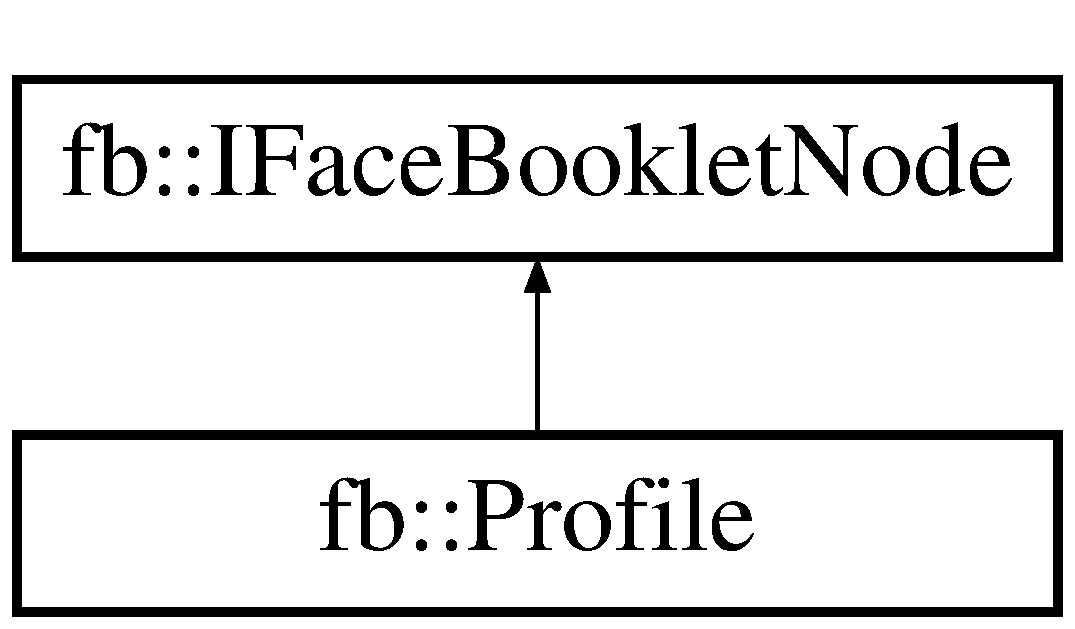
\includegraphics[height=2.000000cm]{classfb_1_1_profile}
\end{center}
\end{figure}
\subsection*{Public Member Functions}
\begin{DoxyCompactItemize}
\item 
\hypertarget{classfb_1_1_profile_a42a0625bef011a0280735db1340e7235}{{\bfseries Profile} (\hyperlink{classfb_1_1_database}{Database} $\ast$db, std\+::string const \&name, \hyperlink{structfb_1_1_date}{Date} const \&birthday=\hyperlink{structfb_1_1_date}{Date}(), time\+\_\+t time=0)}\label{classfb_1_1_profile_a42a0625bef011a0280735db1340e7235}

\item 
const id\+\_\+t \hyperlink{classfb_1_1_profile_aee2df153f7923d0d5c24eb3c11dfff67}{get\+\_\+id} () const 
\begin{DoxyCompactList}\small\item\em getter for booklet's id tag \end{DoxyCompactList}\item 
void \hyperlink{classfb_1_1_profile_a8fe32885a03ac7c92675ede58a230f34}{set\+\_\+id} (id\+\_\+t id)
\begin{DoxyCompactList}\small\item\em setter for booklet's id tag. \end{DoxyCompactList}\item 
std\+::string const \hyperlink{classfb_1_1_profile_a657f6cab3f2caee6fc4b9c8758a711b3}{describe} () const 
\begin{DoxyCompactList}\small\item\em get node's description. \end{DoxyCompactList}\item 
\hyperlink{structfb_1_1_i_face_booklet_node}{I\+Face\+Booklet\+Node} const $\ast$ \hyperlink{classfb_1_1_profile_abd95cad4820c261601b20372f634bd2a}{get\+\_\+friend} (id\+\_\+t id) const 
\begin{DoxyCompactList}\small\item\em retrieves a friend by id number. \end{DoxyCompactList}\item 
\hyperlink{structfb_1_1_i_face_booklet_node}{I\+Face\+Booklet\+Node} $\ast$ \hyperlink{classfb_1_1_profile_a6c9f78b9cb0c1e30d22d17265736a956}{get\+\_\+friend} (id\+\_\+t fr\+\_\+id)
\begin{DoxyCompactList}\small\item\em retrieves a friend by id number. const method. \end{DoxyCompactList}\item 
\hypertarget{classfb_1_1_profile_a2090dc97786cb7cbabf2edf5065b0ddc}{void \hyperlink{classfb_1_1_profile_a2090dc97786cb7cbabf2edf5065b0ddc}{add\+\_\+friend} (\hyperlink{structfb_1_1_i_face_booklet_node}{I\+Face\+Booklet\+Node} $\ast$fr)}\label{classfb_1_1_profile_a2090dc97786cb7cbabf2edf5065b0ddc}

\begin{DoxyCompactList}\small\item\em add a friend to node's friend list \end{DoxyCompactList}\item 
\hypertarget{classfb_1_1_profile_a45472768709c2eb8665ce6e50e2fb5ce}{void {\bfseries remove\+\_\+friend} (id\+\_\+t id)}\label{classfb_1_1_profile_a45472768709c2eb8665ce6e50e2fb5ce}

\item 
\hypertarget{classfb_1_1_profile_a6a579e8b0adade2c3cd499882cf473fc}{\hyperlink{classfb_1_1_node_data}{Node\+Data} \& {\bfseries get\+\_\+data} ()}\label{classfb_1_1_profile_a6a579e8b0adade2c3cd499882cf473fc}

\item 
\hypertarget{classfb_1_1_profile_abc344e9cdafc14dafdaa74678a3cfa48}{\hyperlink{classfb_1_1_node_data}{Node\+Data} const \& {\bfseries get\+\_\+data} () const }\label{classfb_1_1_profile_abc344e9cdafc14dafdaa74678a3cfa48}

\item 
\hypertarget{classfb_1_1_profile_a278304ec0bd7b0f079292069da3cf46f}{void {\bfseries set\+\_\+data} (\hyperlink{classfb_1_1_node_data}{Node\+Data} const \&data)}\label{classfb_1_1_profile_a278304ec0bd7b0f079292069da3cf46f}

\item 
const bool \hyperlink{classfb_1_1_profile_a5f74385d661e8923dd5e66faf35247d7}{has\+\_\+friend} (id\+\_\+t id) const 
\begin{DoxyCompactList}\small\item\em indicates if a node has a given friend. \end{DoxyCompactList}\item 
const bool \hyperlink{classfb_1_1_profile_abe318da2aba42f412dc7373057aa983b}{has\+\_\+friend} (\hyperlink{structfb_1_1_i_face_booklet_node}{I\+Face\+Booklet\+Node} $\ast$node) const 
\begin{DoxyCompactList}\small\item\em indicates if a node has a given friend. \end{DoxyCompactList}\item 
\hypertarget{classfb_1_1_profile_a486c8d589a51ca28dcef95d05aa04dce}{\hyperlink{structfb_1_1_date}{Date} const \& {\bfseries get\+\_\+birthday} () const }\label{classfb_1_1_profile_a486c8d589a51ca28dcef95d05aa04dce}

\item 
\hypertarget{classfb_1_1_profile_a9f2b34badc4cce972e6d47e5a9be508b}{void {\bfseries set\+\_\+birthday} (\hyperlink{structfb_1_1_date}{Date} const \&birthday)}\label{classfb_1_1_profile_a9f2b34badc4cce972e6d47e5a9be508b}

\item 
\hypertarget{classfb_1_1_profile_a586b14f04694abe0860be3e50e6fa706}{virtual \hyperlink{structfb_1_1_i_face_booklet_node}{I\+Face\+Booklet\+Node} $\ast$ \hyperlink{classfb_1_1_profile_a586b14f04694abe0860be3e50e6fa706}{heap\+\_\+copy} ()}\label{classfb_1_1_profile_a586b14f04694abe0860be3e50e6fa706}

\begin{DoxyCompactList}\small\item\em return copy of the node to the heap.  used as a convenience method for copying nodes without knowing their concrete type \end{DoxyCompactList}\end{DoxyCompactItemize}


\subsection{Detailed Description}
Facebooklet profile class. 

Represents a user


\begin{DoxyParams}{Parameters}
{\em db} & pointer to the database which the object will be added to \\
\hline
{\em name} & user name \\
\hline
{\em birthday} & user birthday \\
\hline
{\em time} & time of creation. \\
\hline
\end{DoxyParams}


\subsection{Member Function Documentation}
\hypertarget{classfb_1_1_profile_a657f6cab3f2caee6fc4b9c8758a711b3}{\index{fb\+::\+Profile@{fb\+::\+Profile}!describe@{describe}}
\index{describe@{describe}!fb\+::\+Profile@{fb\+::\+Profile}}
\subsubsection[{describe}]{\setlength{\rightskip}{0pt plus 5cm}string const fb\+::\+Profile\+::describe (
\begin{DoxyParamCaption}
{}
\end{DoxyParamCaption}
) const\hspace{0.3cm}{\ttfamily [virtual]}}}\label{classfb_1_1_profile_a657f6cab3f2caee6fc4b9c8758a711b3}


get node's description. 

Used for printing to std\+::ostream 

Implements \hyperlink{structfb_1_1_i_face_booklet_node_a4ccb08dfa3ae0af8836cec58f8439adc}{fb\+::\+I\+Face\+Booklet\+Node}.

\hypertarget{classfb_1_1_profile_abd95cad4820c261601b20372f634bd2a}{\index{fb\+::\+Profile@{fb\+::\+Profile}!get\+\_\+friend@{get\+\_\+friend}}
\index{get\+\_\+friend@{get\+\_\+friend}!fb\+::\+Profile@{fb\+::\+Profile}}
\subsubsection[{get\+\_\+friend}]{\setlength{\rightskip}{0pt plus 5cm}{\bf I\+Face\+Booklet\+Node} const $\ast$ fb\+::\+Profile\+::get\+\_\+friend (
\begin{DoxyParamCaption}
\item[{id\+\_\+t}]{id}
\end{DoxyParamCaption}
) const\hspace{0.3cm}{\ttfamily [virtual]}}}\label{classfb_1_1_profile_abd95cad4820c261601b20372f634bd2a}


retrieves a friend by id number. 

const method


\begin{DoxyParams}{Parameters}
{\em id} & id of friend \\
\hline
\end{DoxyParams}
\begin{DoxyReturn}{Returns}
pointer to friend node, or if id is not a friend, a nullptr 
\end{DoxyReturn}


Implements \hyperlink{structfb_1_1_i_face_booklet_node_a3a1b982ac4239e23c2204c7746dc90f0}{fb\+::\+I\+Face\+Booklet\+Node}.

\hypertarget{classfb_1_1_profile_a6c9f78b9cb0c1e30d22d17265736a956}{\index{fb\+::\+Profile@{fb\+::\+Profile}!get\+\_\+friend@{get\+\_\+friend}}
\index{get\+\_\+friend@{get\+\_\+friend}!fb\+::\+Profile@{fb\+::\+Profile}}
\subsubsection[{get\+\_\+friend}]{\setlength{\rightskip}{0pt plus 5cm}{\bf I\+Face\+Booklet\+Node} $\ast$ fb\+::\+Profile\+::get\+\_\+friend (
\begin{DoxyParamCaption}
\item[{id\+\_\+t}]{fr\+\_\+id}
\end{DoxyParamCaption}
)\hspace{0.3cm}{\ttfamily [virtual]}}}\label{classfb_1_1_profile_a6c9f78b9cb0c1e30d22d17265736a956}


retrieves a friend by id number. const method. 

const method


\begin{DoxyParams}{Parameters}
{\em id} & id of friend \\
\hline
\end{DoxyParams}
\begin{DoxyReturn}{Returns}
pointer to friend node, or if id is not a friend, a nullptr 
\end{DoxyReturn}


Implements \hyperlink{structfb_1_1_i_face_booklet_node_ae78da353e70e25f3fac8976618bfcde8}{fb\+::\+I\+Face\+Booklet\+Node}.

\hypertarget{classfb_1_1_profile_aee2df153f7923d0d5c24eb3c11dfff67}{\index{fb\+::\+Profile@{fb\+::\+Profile}!get\+\_\+id@{get\+\_\+id}}
\index{get\+\_\+id@{get\+\_\+id}!fb\+::\+Profile@{fb\+::\+Profile}}
\subsubsection[{get\+\_\+id}]{\setlength{\rightskip}{0pt plus 5cm}const id\+\_\+t fb\+::\+Profile\+::get\+\_\+id (
\begin{DoxyParamCaption}
{}
\end{DoxyParamCaption}
) const\hspace{0.3cm}{\ttfamily [virtual]}}}\label{classfb_1_1_profile_aee2df153f7923d0d5c24eb3c11dfff67}


getter for booklet's id tag 

\begin{DoxyReturn}{Returns}
id value 
\end{DoxyReturn}


Implements \hyperlink{structfb_1_1_i_face_booklet_node_a651a6fb7445f8d2c046066c1d381f424}{fb\+::\+I\+Face\+Booklet\+Node}.

\hypertarget{classfb_1_1_profile_a5f74385d661e8923dd5e66faf35247d7}{\index{fb\+::\+Profile@{fb\+::\+Profile}!has\+\_\+friend@{has\+\_\+friend}}
\index{has\+\_\+friend@{has\+\_\+friend}!fb\+::\+Profile@{fb\+::\+Profile}}
\subsubsection[{has\+\_\+friend}]{\setlength{\rightskip}{0pt plus 5cm}const bool fb\+::\+Profile\+::has\+\_\+friend (
\begin{DoxyParamCaption}
\item[{id\+\_\+t}]{id}
\end{DoxyParamCaption}
) const\hspace{0.3cm}{\ttfamily [virtual]}}}\label{classfb_1_1_profile_a5f74385d661e8923dd5e66faf35247d7}


indicates if a node has a given friend. 


\begin{DoxyParams}{Parameters}
{\em id} & id key for friend\\
\hline
\end{DoxyParams}
\begin{DoxyReturn}{Returns}
true if id corresponds to the node's friend 
\end{DoxyReturn}


Implements \hyperlink{structfb_1_1_i_face_booklet_node_a2692d3ad9e903bd545c7074c710e5cdc}{fb\+::\+I\+Face\+Booklet\+Node}.

\hypertarget{classfb_1_1_profile_abe318da2aba42f412dc7373057aa983b}{\index{fb\+::\+Profile@{fb\+::\+Profile}!has\+\_\+friend@{has\+\_\+friend}}
\index{has\+\_\+friend@{has\+\_\+friend}!fb\+::\+Profile@{fb\+::\+Profile}}
\subsubsection[{has\+\_\+friend}]{\setlength{\rightskip}{0pt plus 5cm}const bool fb\+::\+Profile\+::has\+\_\+friend (
\begin{DoxyParamCaption}
\item[{{\bf I\+Face\+Booklet\+Node} $\ast$}]{node}
\end{DoxyParamCaption}
) const\hspace{0.3cm}{\ttfamily [virtual]}}}\label{classfb_1_1_profile_abe318da2aba42f412dc7373057aa983b}


indicates if a node has a given friend. 


\begin{DoxyParams}{Parameters}
{\em node} & pointer to a \hyperlink{structfb_1_1_i_face_booklet_node}{I\+Face\+Booklet\+Node}\\
\hline
\end{DoxyParams}
\begin{DoxyReturn}{Returns}
true if node corresponds to the node's friend 
\end{DoxyReturn}


Implements \hyperlink{structfb_1_1_i_face_booklet_node_af821de82c96e235108ca909a92838dc1}{fb\+::\+I\+Face\+Booklet\+Node}.

\hypertarget{classfb_1_1_profile_a8fe32885a03ac7c92675ede58a230f34}{\index{fb\+::\+Profile@{fb\+::\+Profile}!set\+\_\+id@{set\+\_\+id}}
\index{set\+\_\+id@{set\+\_\+id}!fb\+::\+Profile@{fb\+::\+Profile}}
\subsubsection[{set\+\_\+id}]{\setlength{\rightskip}{0pt plus 5cm}void fb\+::\+Profile\+::set\+\_\+id (
\begin{DoxyParamCaption}
\item[{id\+\_\+t}]{id}
\end{DoxyParamCaption}
)\hspace{0.3cm}{\ttfamily [virtual]}}}\label{classfb_1_1_profile_a8fe32885a03ac7c92675ede58a230f34}


setter for booklet's id tag. 

this should be used with caution, as all other relationships depend on node ids. It is probably best to handle id modifications in the host database instance.


\begin{DoxyParams}{Parameters}
{\em id} & id number to set \\
\hline
\end{DoxyParams}


Implements \hyperlink{structfb_1_1_i_face_booklet_node_a944a07a514d6c88414c533dc7be3193d}{fb\+::\+I\+Face\+Booklet\+Node}.



The documentation for this class was generated from the following files\+:\begin{DoxyCompactItemize}
\item 
/\+Users/\+Shea/\+Documents/school/cmps/facebooklet/src/\hyperlink{_f_b_profile_8h}{F\+B\+Profile.\+h}\item 
/\+Users/\+Shea/\+Documents/school/cmps/facebooklet/src/F\+B\+Profile.\+cc\end{DoxyCompactItemize}

\hypertarget{classfb_1_1_prompter}{\section{fb\+:\+:Prompter$<$ I\+S\+T\+R\+E\+A\+M\+\_\+\+T $>$ Class Template Reference}
\label{classfb_1_1_prompter}\index{fb\+::\+Prompter$<$ I\+S\+T\+R\+E\+A\+M\+\_\+\+T $>$@{fb\+::\+Prompter$<$ I\+S\+T\+R\+E\+A\+M\+\_\+\+T $>$}}
}


template class for prompting user for data  




{\ttfamily \#include $<$Face\+Booklet.\+h$>$}

\subsection*{Public Member Functions}
\begin{DoxyCompactItemize}
\item 
\hypertarget{classfb_1_1_prompter_af0270c9ee1234d8ed892e4137c3e225a}{{\bfseries Prompter} (I\+S\+T\+R\+E\+A\+M\+\_\+\+T \&in)}\label{classfb_1_1_prompter_af0270c9ee1234d8ed892e4137c3e225a}

\item 
\hyperlink{classfb_1_1_profile}{Profile} $\ast$ \hyperlink{classfb_1_1_prompter_acc93a31b8d47be2358ff044cb2ee9521}{create\+\_\+profile} (\hyperlink{classfb_1_1_database}{Database} $\ast$db)
\begin{DoxyCompactList}\small\item\em generates a new profile \end{DoxyCompactList}\end{DoxyCompactItemize}
\subsection*{Public Attributes}
\begin{DoxyCompactItemize}
\item 
\hypertarget{classfb_1_1_prompter_a2f77a9922842a56959b65fecc5d11e0a}{I\+S\+T\+R\+E\+A\+M\+\_\+\+T \& {\bfseries in}}\label{classfb_1_1_prompter_a2f77a9922842a56959b65fecc5d11e0a}

\end{DoxyCompactItemize}


\subsection{Detailed Description}
\subsubsection*{template$<$typename I\+S\+T\+R\+E\+A\+M\+\_\+\+T = std\+::istream$>$class fb\+::\+Prompter$<$ I\+S\+T\+R\+E\+A\+M\+\_\+\+T $>$}

template class for prompting user for data 

Implemented as a template class for generic i/o streams. Allows automated testing of prompter with string streams


\begin{DoxyTemplParams}{Template Parameters}
{\em I\+S\+T\+R\+E\+A\+M\+\_\+\+T=std\+::istream} & an input stream S\+T\+L type \\
\hline
\end{DoxyTemplParams}


\subsection{Member Function Documentation}
\hypertarget{classfb_1_1_prompter_acc93a31b8d47be2358ff044cb2ee9521}{\index{fb\+::\+Prompter@{fb\+::\+Prompter}!create\+\_\+profile@{create\+\_\+profile}}
\index{create\+\_\+profile@{create\+\_\+profile}!fb\+::\+Prompter@{fb\+::\+Prompter}}
\subsubsection[{create\+\_\+profile}]{\setlength{\rightskip}{0pt plus 5cm}template$<$typename I\+S\+T\+R\+E\+A\+M\+\_\+\+T = std\+::istream$>$ {\bf Profile}$\ast$ {\bf fb\+::\+Prompter}$<$ I\+S\+T\+R\+E\+A\+M\+\_\+\+T $>$\+::create\+\_\+profile (
\begin{DoxyParamCaption}
\item[{{\bf Database} $\ast$}]{db}
\end{DoxyParamCaption}
)\hspace{0.3cm}{\ttfamily [inline]}}}\label{classfb_1_1_prompter_acc93a31b8d47be2358ff044cb2ee9521}


generates a new profile 


\begin{DoxyParams}{Parameters}
{\em db} & pointer to the database object \\
\hline
\end{DoxyParams}
\begin{DoxyReturn}{Returns}
a pointer to the new profile, added to the database 
\end{DoxyReturn}


The documentation for this class was generated from the following file\+:\begin{DoxyCompactItemize}
\item 
/\+Users/\+Shea/\+Documents/school/cmps/facebooklet/src/\hyperlink{_face_booklet_8h}{Face\+Booklet.\+h}\end{DoxyCompactItemize}

\chapter{File Documentation}
\hypertarget{_date_8h}{\section{/\+Users/\+Shea/cmps/facebooklet/src/\+Date.h File Reference}
\label{_date_8h}\index{/\+Users/\+Shea/cmps/facebooklet/src/\+Date.\+h@{/\+Users/\+Shea/cmps/facebooklet/src/\+Date.\+h}}
}


Date structure type.  


{\ttfamily \#include $<$time.\+h$>$}\\*
\subsection*{Classes}
\begin{DoxyCompactItemize}
\item 
struct \hyperlink{structfb_1_1_date}{fb\+::\+Date}
\begin{DoxyCompactList}\small\item\em \hyperlink{structfb_1_1_date}{Date} data structure. \end{DoxyCompactList}\end{DoxyCompactItemize}
\subsection*{Enumerations}
\begin{DoxyCompactItemize}
\item 
enum {\bfseries Month} \{ \\*
{\bfseries Jan} = 1, 
{\bfseries Feb}, 
{\bfseries Mar}, 
{\bfseries Apr}, 
\\*
{\bfseries May}, 
{\bfseries Jun}, 
{\bfseries Jul}, 
{\bfseries Aug}, 
\\*
{\bfseries Sep}, 
{\bfseries Oct}, 
{\bfseries Nov}, 
{\bfseries Dec}
 \}
\begin{DoxyCompactList}\small\item\em enum class for Month values \end{DoxyCompactList}\end{DoxyCompactItemize}
\subsection*{Functions}
\begin{DoxyCompactItemize}
\item 
\hypertarget{namespacefb_a787dd35a17507c9852a818bca6382499}{bool {\bfseries fb\+::operator==} (Date const \&lhs, Date const \&rhs)}\label{namespacefb_a787dd35a17507c9852a818bca6382499}

\end{DoxyCompactItemize}


\subsection{Detailed Description}
Date structure type. 

Created by Steven on 4/18/15. 
\hypertarget{_face_booklet_8h}{\section{/\+Users/\+Shea/cmps/facebooklet/src/\+Face\+Booklet.h File Reference}
\label{_face_booklet_8h}\index{/\+Users/\+Shea/cmps/facebooklet/src/\+Face\+Booklet.\+h@{/\+Users/\+Shea/cmps/facebooklet/src/\+Face\+Booklet.\+h}}
}


defines main Facebooklet class  


{\ttfamily \#include $<$iostream$>$}\\*
{\ttfamily \#include \char`\"{}F\+B\+Profile.\+h\char`\"{}}\\*
{\ttfamily \#include \char`\"{}Date.\+h\char`\"{}}\\*
\subsection*{Classes}
\begin{DoxyCompactItemize}
\item 
class \hyperlink{classfb_1_1_prompter}{fb\+::\+Prompter}
\begin{DoxyCompactList}\small\item\em template class for prompting user for data \end{DoxyCompactList}\item 
class \hyperlink{classfb_1_1_face_booklet}{fb\+::\+Face\+Booklet}
\begin{DoxyCompactList}\small\item\em main function for \hyperlink{classfb_1_1_face_booklet}{Face\+Booklet} program. \end{DoxyCompactList}\end{DoxyCompactItemize}
\subsection*{Enumerations}
\begin{DoxyCompactItemize}
\item 
\hypertarget{namespacefb_a1d613b526849fecad2e0906c77654e23}{enum {\bfseries Menu\+Opt} \{ \\*
{\bfseries create\+Profile}, 
{\bfseries login}, 
{\bfseries view\+Profile}, 
{\bfseries quit}, 
\\*
{\bfseries add\+Friend}, 
{\bfseries rem\+Friend}, 
{\bfseries post}
 \}}\label{namespacefb_a1d613b526849fecad2e0906c77654e23}

\begin{DoxyCompactList}\small\item\em enum class for options available to main menu \end{DoxyCompactList}\end{DoxyCompactItemize}


\subsection{Detailed Description}
defines main Facebooklet class 

declarations for the prompter and main Facebooklet class.

Steve Shea

Steve Shea

For this project, I have chosen to roughly emulate a model-\/view-\/controller architecture as a way of separating concerns of the various classes. The I\+Facebooklet\+Node, Profile, Database, and Node\+Data classes make up the model by manipulating and storing data. The Prompter class handles user input. It is given instructions from the Facebooklet instance, and provides promts and parses input. Rather than using std\+::cin dirrectly, it takes a std\+::istream object reference. This allows for easier testing, as you can pass in a stringstream object to emulate user input (this can be seen in the test cases of test/engine\+\_\+tests.\+c). Finally, The Facebooklet class acts as the controller. It provides an interface between the model and the user interactions handled by Prompter, such as adding users or posts. It also provides the program's main loop method. 
\hypertarget{_f_b_profile_8h}{\section{/\+Users/\+Shea/cmps/facebooklet/src/\+F\+B\+Profile.h File Reference}
\label{_f_b_profile_8h}\index{/\+Users/\+Shea/cmps/facebooklet/src/\+F\+B\+Profile.\+h@{/\+Users/\+Shea/cmps/facebooklet/src/\+F\+B\+Profile.\+h}}
}


definition for concrete Profile type  


{\ttfamily \#include \char`\"{}interfaces.\+h\char`\"{}}\\*
{\ttfamily \#include \char`\"{}Database.\+h\char`\"{}}\\*
{\ttfamily \#include \char`\"{}utils.\+h\char`\"{}}\\*
{\ttfamily \#include \char`\"{}Date.\+h\char`\"{}}\\*
{\ttfamily \#include $<$set$>$}\\*
{\ttfamily \#include $<$map$>$}\\*
\subsection*{Classes}
\begin{DoxyCompactItemize}
\item 
class \hyperlink{classfb_1_1_profile}{fb\+::\+Profile}
\begin{DoxyCompactList}\small\item\em Facebooklet profile class. \end{DoxyCompactList}\end{DoxyCompactItemize}


\subsection{Detailed Description}
definition for concrete Profile type 

Steve Shea 
\hypertarget{interfaces_8h}{\section{/\+Users/\+Shea/cmps/facebooklet/src/interfaces.h File Reference}
\label{interfaces_8h}\index{/\+Users/\+Shea/cmps/facebooklet/src/interfaces.\+h@{/\+Users/\+Shea/cmps/facebooklet/src/interfaces.\+h}}
}


defines interface type for Facebooklet Nodes  


{\ttfamily \#include $<$string$>$}\\*
{\ttfamily \#include $<$iostream$>$}\\*
{\ttfamily \#include $<$memory$>$}\\*
{\ttfamily \#include $<$vector$>$}\\*
{\ttfamily \#include \char`\"{}utils.\+h\char`\"{}}\\*
{\ttfamily \#include \char`\"{}Node\+Data.\+h\char`\"{}}\\*
\subsection*{Classes}
\begin{DoxyCompactItemize}
\item 
struct \hyperlink{structfb_1_1_i_face_booklet_node}{fb\+::\+I\+Face\+Booklet\+Node}
\begin{DoxyCompactList}\small\item\em interface class for \hyperlink{classfb_1_1_face_booklet}{Face\+Booklet} nodes \end{DoxyCompactList}\end{DoxyCompactItemize}
\subsection*{Typedefs}
\begin{DoxyCompactItemize}
\item 
using {\bfseries fb\+::\+Node\+Uptr} = std\+::unique\+\_\+ptr$<$ I\+Face\+Booklet\+Node $>$
\item 
\hypertarget{namespacefb_ac37445a0066ef77ee7888b8b9f9f4061}{using {\bfseries fb\+::\+Node\+Sptr} = std\+::shared\+\_\+ptr$<$ I\+Face\+Booklet\+Node $>$}\label{namespacefb_ac37445a0066ef77ee7888b8b9f9f4061}

\item 
\hypertarget{namespacefb_afa2072c032827f99751b2409abae7c5e}{using {\bfseries fb\+::\+Node\+Wptr} = std\+::weak\+\_\+ptr$<$ I\+Face\+Booklet\+Node $>$}\label{namespacefb_afa2072c032827f99751b2409abae7c5e}

\end{DoxyCompactItemize}
\subsection*{Functions}
\begin{DoxyCompactItemize}
\item 
\hypertarget{namespacefb_a98bb841108489aaed3daffc115c5e059}{bool {\bfseries fb\+::operator==} (I\+Face\+Booklet\+Node const \&self, I\+Face\+Booklet\+Node const \&rhs)}\label{namespacefb_a98bb841108489aaed3daffc115c5e059}

\end{DoxyCompactItemize}


\subsection{Detailed Description}
defines interface type for Facebooklet Nodes 

Steve Shea 
\hypertarget{_node_data_8h}{\section{/\+Users/\+Shea/\+Documents/school/cmps/facebooklet/src/\+Node\+Data.h File Reference}
\label{_node_data_8h}\index{/\+Users/\+Shea/\+Documents/school/cmps/facebooklet/src/\+Node\+Data.\+h@{/\+Users/\+Shea/\+Documents/school/cmps/facebooklet/src/\+Node\+Data.\+h}}
}


contains data for building node data  


{\ttfamily \#include $<$string$>$}\\*
{\ttfamily \#include $<$vector$>$}\\*
{\ttfamily \#include $<$ctime$>$}\\*
{\ttfamily \#include \char`\"{}utils.\+h\char`\"{}}\\*
\subsection*{Classes}
\begin{DoxyCompactItemize}
\item 
struct \hyperlink{structfb_1_1_node_post}{fb\+::\+Node\+Post}
\begin{DoxyCompactList}\small\item\em Record type for storing data of a single post. \end{DoxyCompactList}\item 
class \hyperlink{classfb_1_1_node_data}{fb\+::\+Node\+Data}
\begin{DoxyCompactList}\small\item\em the class containing a node's basic information and post history. \end{DoxyCompactList}\end{DoxyCompactItemize}
\subsection*{Functions}
\begin{DoxyCompactItemize}
\item 
\hypertarget{namespacefb_a52381fb6caae5d9692cb1fbc562d99ac}{bool {\bfseries fb\+::operator==} (Node\+Post const \&lhs, Node\+Post const \&rhs)}\label{namespacefb_a52381fb6caae5d9692cb1fbc562d99ac}

\begin{DoxyCompactList}\small\item\em equality operator for \hyperlink{structfb_1_1_node_post}{Node\+Post} \end{DoxyCompactList}\item 
\hypertarget{namespacefb_a8555f271f88c0ace7024ad073ee7d327}{bool {\bfseries fb\+::operator==} (Node\+Data const \&lhs, Node\+Data const \&rhs)}\label{namespacefb_a8555f271f88c0ace7024ad073ee7d327}

\begin{DoxyCompactList}\small\item\em equality operator for \hyperlink{classfb_1_1_node_data}{Node\+Data} \end{DoxyCompactList}\end{DoxyCompactItemize}


\subsection{Detailed Description}
contains data for building node data 

Created by Steven on 4/14/15. 
\hypertarget{utils_8h}{\section{/\+Users/\+Shea/\+Documents/school/cmps/facebooklet/src/utils.h File Reference}
\label{utils_8h}\index{/\+Users/\+Shea/\+Documents/school/cmps/facebooklet/src/utils.\+h@{/\+Users/\+Shea/\+Documents/school/cmps/facebooklet/src/utils.\+h}}
}


utilitiy functions  


\subsection*{Typedefs}
\begin{DoxyCompactItemize}
\item 
\hypertarget{namespacefb_a318c8fb1972ca47e450af7c9f8144c41}{using {\bfseries fb\+::id\+\_\+t} = size\+\_\+t}\label{namespacefb_a318c8fb1972ca47e450af7c9f8144c41}

\begin{DoxyCompactList}\small\item\em typedef of size\+\_\+t, used as id keys for nodes \end{DoxyCompactList}\end{DoxyCompactItemize}


\subsection{Detailed Description}
utilitiy functions 

Created by Steven on 4/14/15. 
%--- End generated contents ---

% Index
\newpage
\phantomsection
\addcontentsline{toc}{chapter}{Index}
\printindex

\end{document}
